% !TeX root = ../../../book.tex

\subsection{示意图}

在深入讨论函数的抽象性质和证明方法之前,我们先介绍一种直观表示函数的方法。需要强调的是,这种方法在数学上并不\emph{严谨},在\emph{证明}中使用可能不够妥当(例如,在评分作业中,即使思路正确,也可能无法获得满分)。然而,它能生动展示函数的工作原理,帮助发现问题并推动更严格的证明。特别地,在构造\emph{反例}以反驳函数性质时,这种方法尤为有效。

\textbf{示意图}的概念类似于用\emph{韦恩图}表示集合。集合本质上是元素的集合,而非纸上的阴影圆圈,但这些视觉元素能辅助理解和描述集合。同样,函数是两个集合间满足特定条件的关系,而非简单的图形表达:

\begin{center}
    {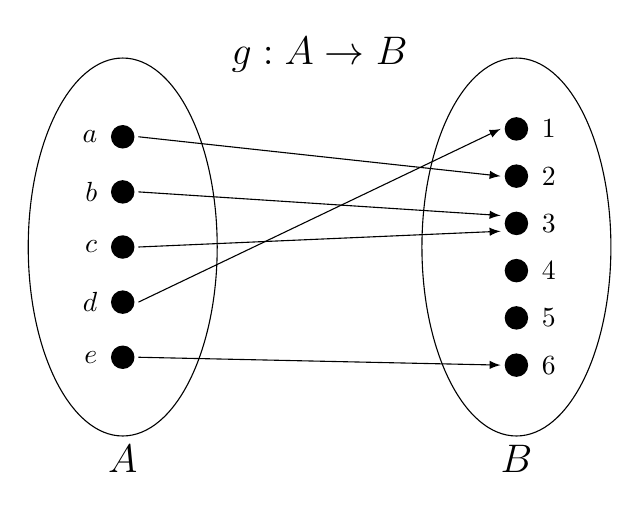
\begin{tikzpicture}[scale=1]
        \foreach \x in {1,...,6}
        {
            \node at (5, -\x*0.6)[circle,fill,inner sep=3pt]{};
            \draw[shift={(5.2, -\x*0.6)}] node[right] {$\x$};
        }
        \draw (5,-2.1) ellipse (1.2 and 2.4);

        \foreach \x/\s in  {1/a,2/b,3/c,4/d,5/e}
        {
            \node at (0, -\x*0.7)[circle,fill,inner sep=3pt]{};
            \draw[shift={(-0.2, -\x*0.7)}] node[left] {$\s$};
        }
        \draw (0,-2.1) ellipse (1.2 and 2.4);

        \draw[-latex] (0.2,-0.7) -- (4.8,-1.2); 
        \draw[-latex] (0.2,-1.4) -- (4.8,-1.7); 
        \draw[-latex] (0.2,-2.1) -- (4.8,-1.9); 
        \draw[-latex] (0.2,-2.8) -- (4.8,-0.6); 
        \draw[-latex] (0.2,-3.5) -- (4.8,-3.6);
        
        \node[below] at (0, -4.5){\Large $A$};
        \node[below] at (5, -4.5){\Large $B$};
        \node[above] at (2.5, 0){\Large $g:A \to B$};
    \end{tikzpicture}}
\end{center}

尽管如此,这种表示确实在某种程度上\emph{体现}了函数的核心思想。图中用椭圆分别标识定义域 $A$ 和值域 $B$,元素以椭圆内的标记点表示。我们根据函数 $g: A \to B$ 在点间绘制箭头。

该方法常用于探索函数特性或构造反例以驳斥某些论断。通过绘制点与箭头并尝试不同的连接方式,我们能逐步构建例子的基本\emph{框架}。随后,为图中元素分配具体名称和公式,使其严谨化。

在后续讨论中,我们将用示意图辅助说明某些属性和概念,同时辅以更严格的陈述或描述。我们鼓励你也采用这一方法。
